\documentclass[12pt,a4paper,UTF8]{ctexart}




%设置页边距
\usepackage{geometry}
\geometry{left=2.5cm,right=2.5cm,top=2.5cm,bottom=2.5cm}




%需要用到的扩展包
\usepackage{xeCJK,amsmath,paralist,enumerate,booktabs,multirow,graphicx,float,subfig,setspace,listings,lastpage,hyperref}
\usepackage{fancyhdr}




%设置页眉页脚以及页码
\pagestyle{fancy}
\rhead{直流双臂电桥}
\lhead{大学基础物理实验报告}
\cfoot{Page\thepage/\pageref{LastPage}}
\rfoot{\today}




%报告中用到的图片存放在这个tex文件所在目录中的figures子目录中
\graphicspath{{figures/}}









%报告开始
\begin{document}
	
	
	
	
	%设置课程标题
	\begin{center}
		\heiti\LARGE{《大学基础物理实验》课程实验报告}
	\end{center}
	
	
	
	
	%设置实验人信息以及实验时间表格


		\begin{center}
			\begin{tabular}{lcr}
				
				{\songti 姓名及学号:蒋丰毅 2211082}  \quad 专业:工科试验班 \quad 年级:22级 \quad 座号:10\\
				{\songti  学院:软件学院 \quad 实验组别:C组\quad 实验时间:2023年4月14日~星期五~上午}\\
				
				
			\end{tabular}
		\end{center}
	\vspace{-0.2cm}
	{\noindent}	 \rule[-10pt]{16cm}{0.05em}\\

	\vspace{-0.4cm}
	
	
	
	
	
	
	%实验题目
	\begin{center}
		\LARGE\textbf{直流双臂电桥}
	\end{center}
	

	
	%实验原理
	\subsection*{[实验原理]}
	\subsubsection*{直流双臂电桥适用范围:}
	\par 直流双臂电桥适用于测量较小的电阻,如QJ44型直流双臂电桥测量范围: 0.1m$\Omega$-11$\Omega$
	\subsubsection*{四端法:}
	\begin{figure}[!htbp]
		\centering
		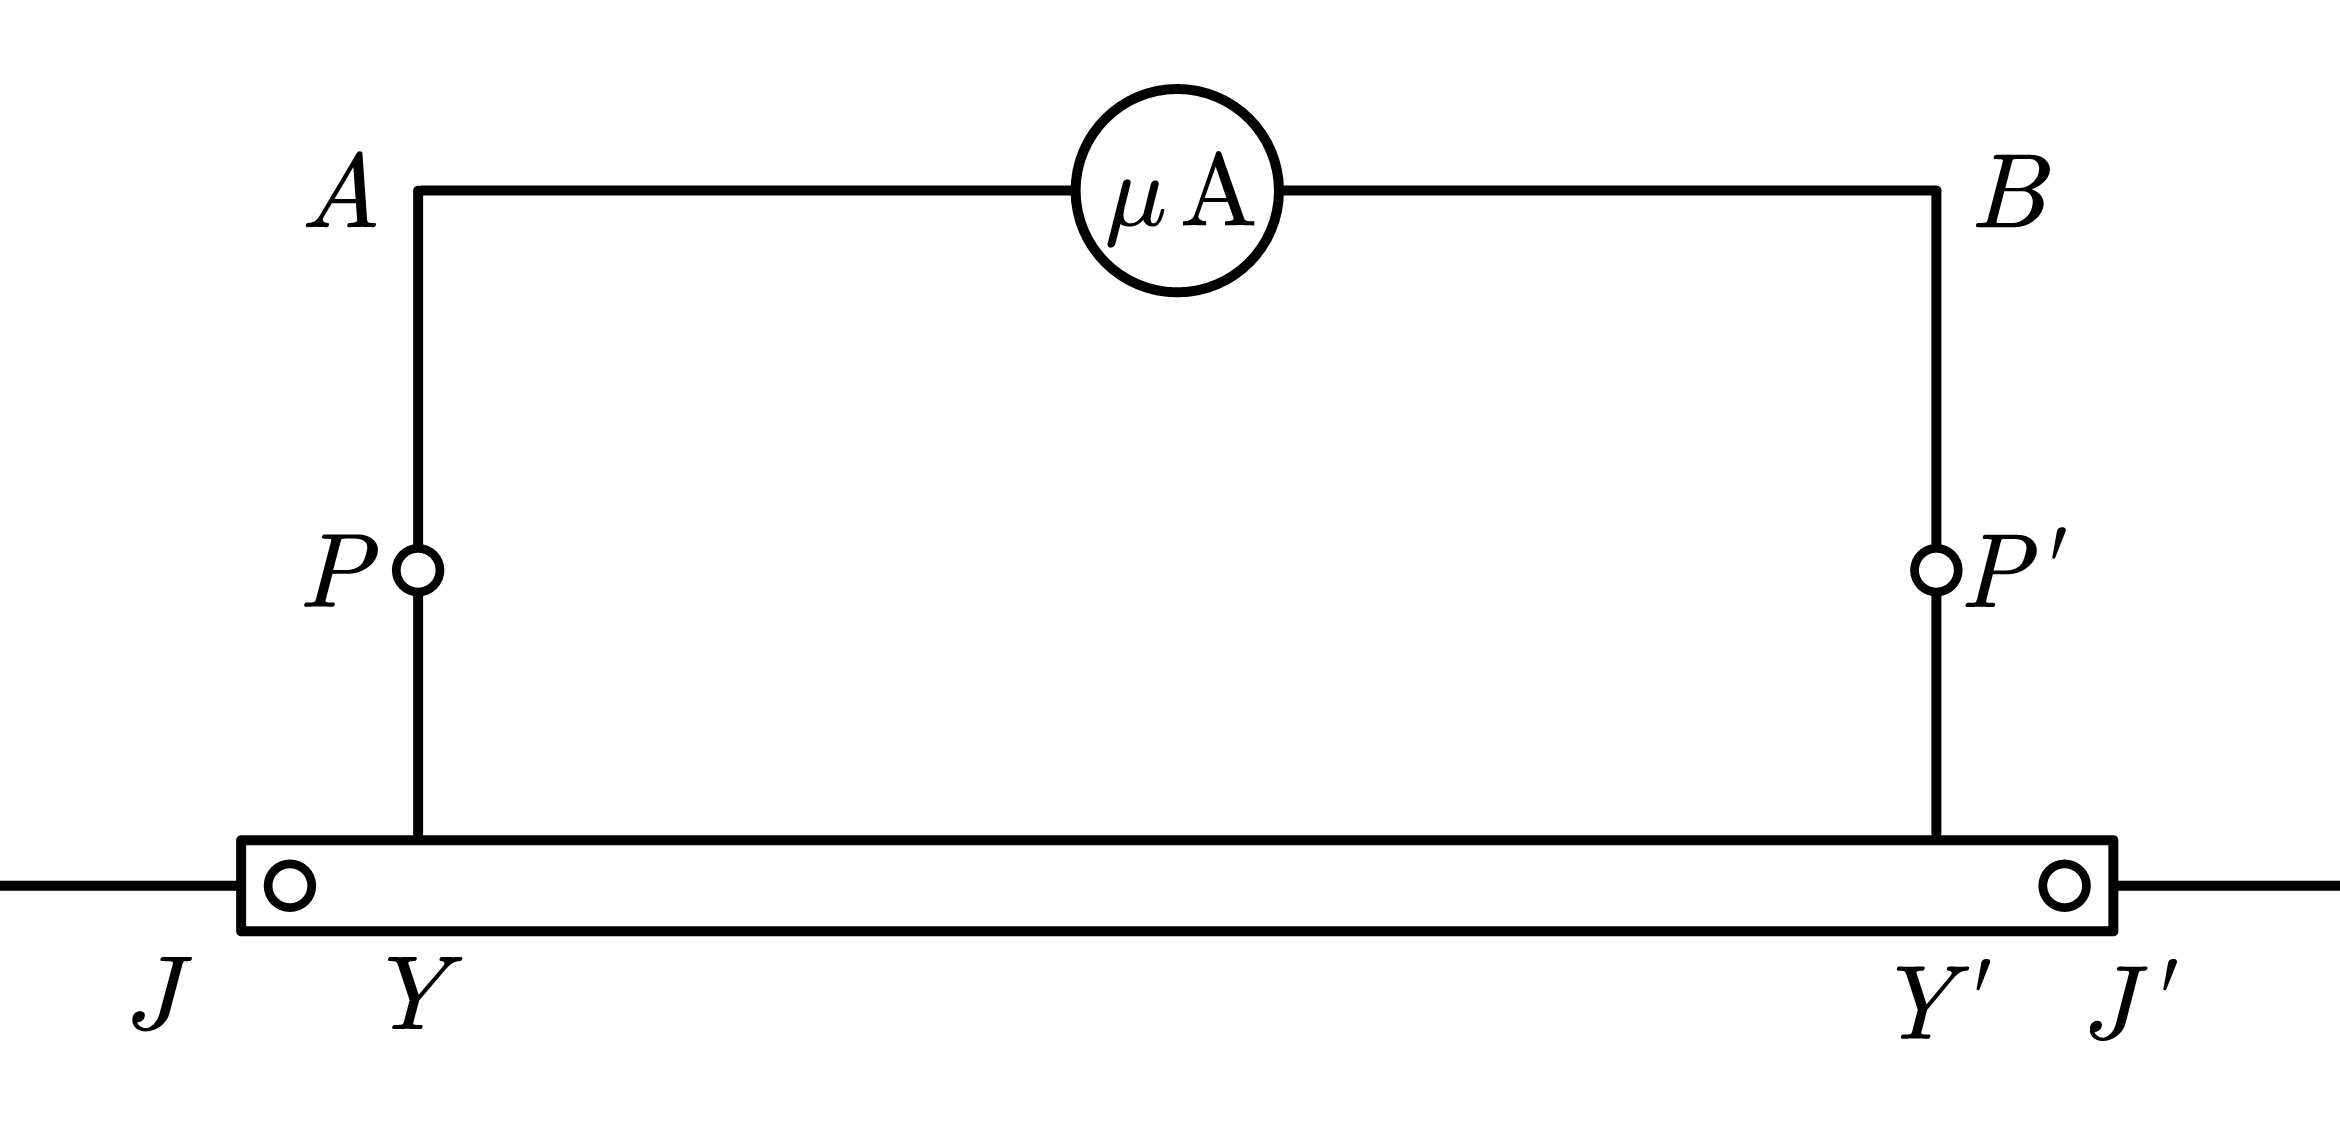
\includegraphics[width=0.6\textwidth]{四端法}
		\caption{四端法原理}
	\end{figure}
	\par 可以看出,使用图1的电路进行测量,在电阻体上$Y,Y^{\prime}$上两个点焊出两个接头再与微安表相连接,这样可以保证微安表所连接两点之间的阻值正好为$Y,Y^{\prime}$之间的阻值,又$A,B,P,P^{\prime}$四个点的接触电阻和$AY,BY^{\prime}$的接线电阻都分给了微安表,保证了分流的精确。由于电阻被做成了四个接头,故称作“四端结构”。
	
	\subsubsection*{实验电路与测量公式推导}
	\par 测量电路如图2(见下页)所示,其中$R_0$为标准低阻,$R_x$为待测低阻。四个比例臂电阻有意做成几十欧姆以上的阻值,因此他们所在桥臂中的接线电阻和接触电阻的影响便可忽略。注意右边的电阻$R$是为了防止电流过大。当电流计指零时,电桥达到平衡。
	\clearpage
	\begin{figure}
		\centering
		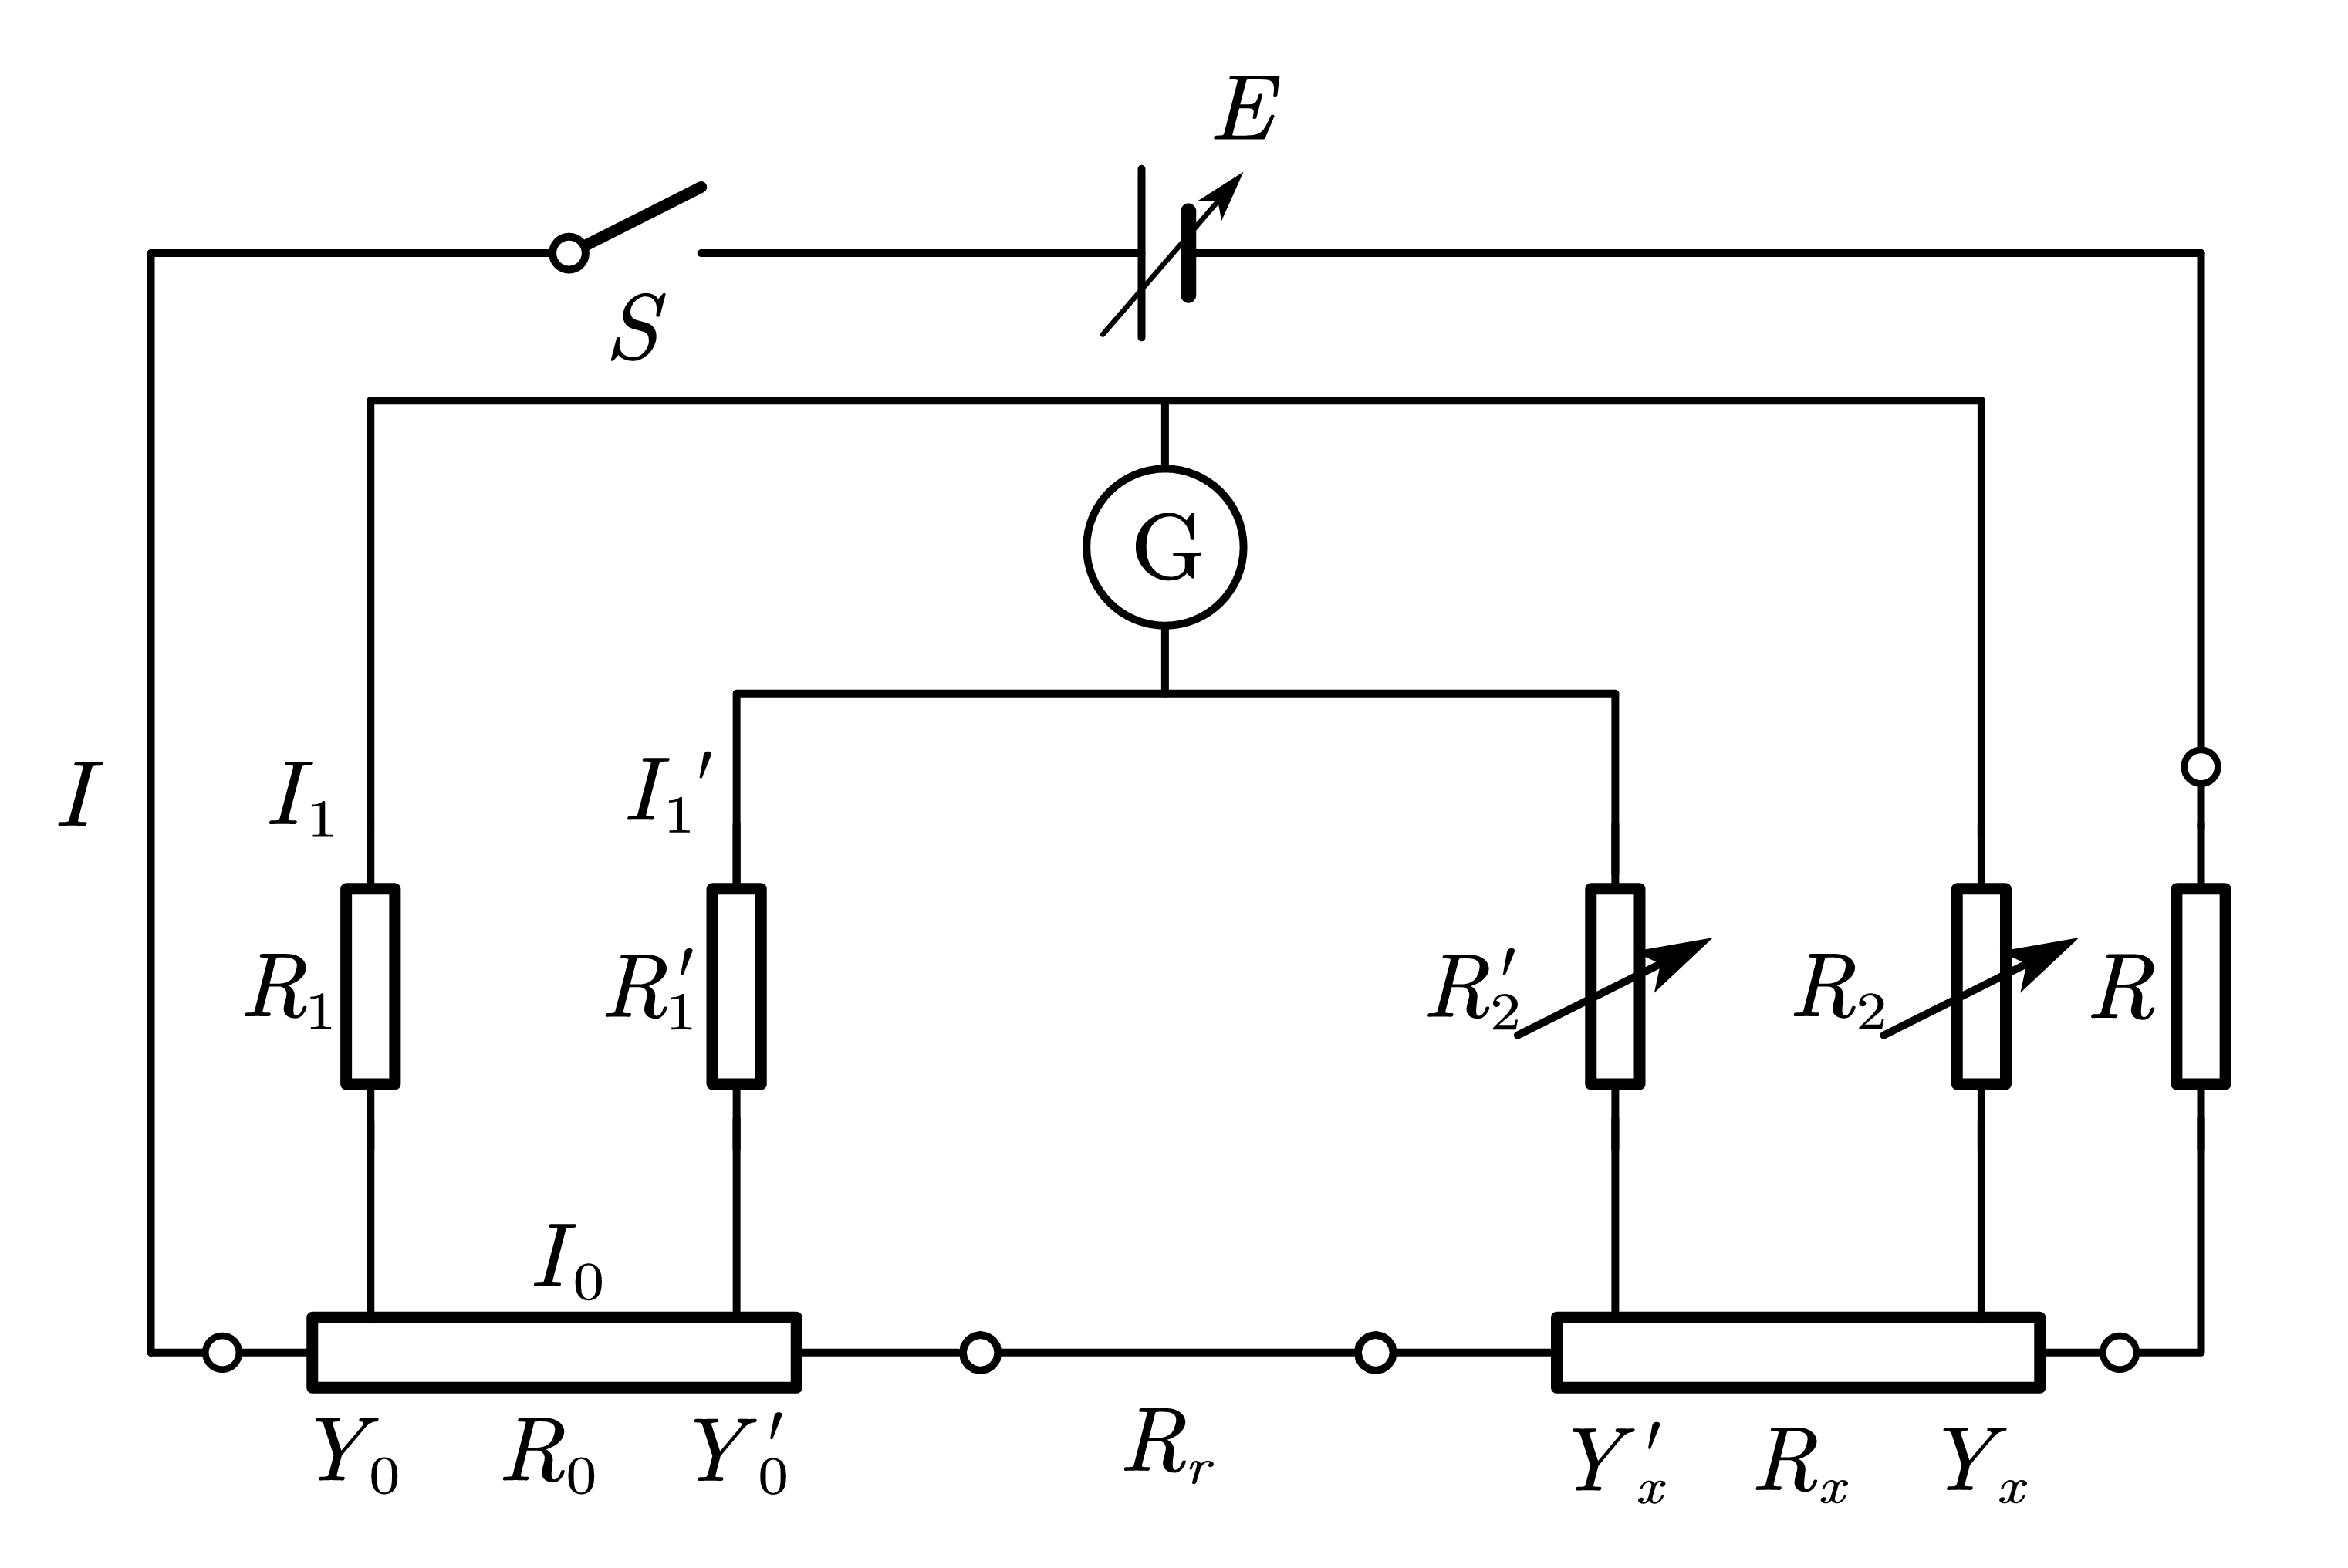
\includegraphics[width=0.6\textwidth]{直流双臂电路图透明}
		\caption{直流双臂电路}
	\end{figure}
	\par 由基尔霍夫定律,可以列出方程组:

	\begin{equation}
		\begin{cases}
			$$I_1 R_1=I_0 R_0+I_1^{\prime} R_1^{\prime} \\
			I_1 R_2=I_0 R_x+I_1^{\prime} R_2^{\prime} \\
			\left(I_0-I_1^{\prime}\right) R_{\mathrm{r}}=I_1^{\prime}\left(R_1^{\prime}+R_2^{\prime}\right)$$
		\end{cases}
	\end{equation}
	\par 式中$I_1,I_0,I_1^{\prime}$分别为图中所标示,将(1)式整理得:
	\[R_{1}R_{x}=R_{2}R_{0}+(\,R_{2}R_{1}^{\prime}-R_{1}R_{2}^{\prime}\,)\,{\frac{r}{R_{r}+R_{1}^{\prime}+R_{2}^{\prime}}}\]
	\par 当电桥的平衡是在保证$R_{2}R_{1}^{\prime}-R_{1}R_{2}^{\prime}=0$的情况下,则上式可以简化为
	\[R_{x}={\frac{R_{2}}{R_{1}}}R_{0}\]
	\par 由此可知此次实验双臂电桥的测量平衡条件为:
	\[{\frac{R_{2}}{{R_{1}}}}={\frac{{R_{2}^{\prime}}}{{R_{1}^{\prime}}}}={\frac{{R_{x}}}{{R_{0}}}}\]
	\par 本次实验使用同步调节比例臂电阻$R_2,R_2^{\prime}$的方法使电流计示零。
	\subsubsection*{双臂电桥灵敏度}
	\par 双臂电桥平衡后将比例臂电阻$R_2,R_2^{\prime}$同步调偏$\Delta R_2=\Delta R_2^{\prime}$,若电流计示数改变$\Delta I$,则灵敏度$S$为:
	\[
	S=\frac{\Delta I}{\Delta R_2 / R_2}
	\]
	\clearpage
	\par 由$S={\dfrac{\Delta I}{\Delta R_{2}/R_{2}}}={\dfrac{\Delta I}{\Delta R_{x}/R_{x}}}$可以引入相对误差:
	$${\frac{\Delta R_{x}}{R_{x}}}={\frac{\Delta I}{S}}$$
	\subsection*{数据处理}
	\subsubsection*{数据记录表}
	
	\begin{table}[!htbp]
		\centering
		\caption{样品阻值测量}
		\begin{tabular}{c|ccc}
			\toprule
			\makebox[0.05\textwidth][c]{X}&\makebox[0.25\textwidth][c]{平衡时:$R_2=R_2^{\prime}(\Omega)$}&\makebox[0.25\textwidth][c]{改变:$\Delta R_2=\Delta R_2^{\prime}(\Omega)$}&\makebox[0.25\textwidth][c]{电流变化:$\Delta I(nA)$}\\
			\midrule
			铜 & 416.2 & 20  & 0.3 \\
			铁 & 16810 & 300 & 1.6 \\
			铝 & 992   & 50  & 2.8\\
			\bottomrule
		\end{tabular}
	\end{table}
	\begin{table}[!htbp]
	\centering
	\caption{样品直径测量}
	\begin{tabular}{ccccccc}
		\toprule
		\makebox[0.1\textwidth][c]{样品(mm)}&\makebox[0.1\textwidth][c]{测量1}&\makebox[0.1\textwidth][c]{测量2}&\makebox[0.1\textwidth][c]{测量3}&\makebox[0.1\textwidth][c]{测量4}&\makebox[0.1\textwidth][c]{测量5}&\makebox[0.15\textwidth][c]{平均}\\
		\midrule
		铜 & 5.45 & 5.44  & 5.45 & 5.43 & 5.44 & 5.442 \\
		铁 & 5.44 & 5.445 & 5.45 & 5.46 & 5.46 & 5.451 \\
		铝 & 5.39 & 5.4   & 5.24 & 5.41 & 5.41 & 5.37\\
		\bottomrule
	\end{tabular}
	\end{table}
	\begin{table}[!htbp]
	\centering
	\caption{样品长度测量}
	\begin{tabular}{cc}
		\toprule
		\makebox[0.15\textwidth][c]{样品}&\makebox[0.15\textwidth][c]{长度L(cm)}\\
		\midrule
		铜 & 46.75\\
		铁 & 46.10\\
		铝 & 46.10\\
		\bottomrule
	\end{tabular}
	\end{table}
	\subsubsection*{电阻率的测量}
	\textbf{长度的不确定度}:由于是单次测量,故只有B类不确定度,假设误差服从均匀分布,已知米尺的允差$\Delta _x$为0.5mm可知:
	\[
	u_l=u_{Bl}=\frac{\Delta_l}{\sqrt{3}}=0.2887(mm)
	\]
	\[E_l = \dfrac{u_l}{l}=\left\{
	\begin{aligned}
		&0.061\%\qquad(Cu)\\ 
		&0.062\%\qquad(Fe)\\
		&0.062\%\qquad(Al)\\
	\end{aligned}
	\right.\]
	\clearpage
	\par 由此可知:三种金属的长度和不确定度分别为
		\begin{table}[!htbp]
		\centering
		\caption{样品长度计算}
		\begin{tabular}{ccc}
			\toprule
			\makebox[0.1\textwidth][c]{样品}&\makebox[0.15\textwidth][c]{长度L(cm)}&\makebox[0.15\textwidth][c]{不确定度(\%)}\\
			\midrule
			铜 & $46.75\pm0.2887$&0.061\\
			铁 & $46.10\pm0.2887$&0.062\\
			铝 & $46.10\pm0.2887$&0.062\\
			\bottomrule
		\end{tabular}
	\end{table}
	\par \textbf{铜棍直径测量}: 由于铜棍直径为多次测量,以0.683为置信概率,A类不确定度为:
	\[
	u_{Ad} = 	\sigma_{\overline{d}}=t_{(0.683,4)}s_{\overline{d}}=1.14s_{\overline{d}}
	=\left\{\begin{aligned}
		& 0.0095\qquad(Cu)\\
		& 0.0102\qquad(Fe)\\
		& 0.0834\qquad(Al)
	\end{aligned}\right. \qquad(mm)
	\]
	\par 其中$s^2_{\overline{d}}=\frac{\sum_{i=1}^{n}(d_i-\overline{d})^2}{n-1}$

	\[
	u_{Bd}=\frac{\varepsilon_d}{\sqrt{3}}=0.0058(mm)
	\]
	\par 从而合成两类不确定度:
	\[
	u_d = \sqrt{u_{Ad}^2+u_{Bd}^2} = \left\{\begin{aligned}
		& 0.0111\qquad(Cu)\\
		& 0.0117\qquad(Fe)\\
		& 0.0836\qquad(Al)
	\end{aligned}\right. \qquad(mm)
	\]
	\[
	E_d = \dfrac{u_d}{d}=\left\{
	\begin{aligned}
	&0.20\%\qquad(Cu)\\ 
	&0.21\%\qquad(Fe)\\
	&1.56\%\qquad(Al)\\
	\end{aligned}
	\right.
	\]
	得到:
		\begin{table}[!htbp]
		\centering
		\caption{样品直径计算}
		\begin{tabular}{ccc}
			\toprule
			\makebox[0.1\textwidth][c]{样品}&\makebox[0.15\textwidth][c]{直径D(mm)}&\makebox[0.15\textwidth][c]{不确定度(\%)}\\
			\midrule
			铜 & $5.44\pm 0.01$&0.20\\
			铁 & $5.45\pm0.01$&0.21\\
			铝 & $5.370\pm0.083$&1.56\\
			\bottomrule
		\end{tabular}
	\end{table}
	\clearpage
	\par \textbf{$R_x$的测量}:给定$R_0=0.001\Omega,R_1=1000\Omega$
	\[R_{\overline{x}}={\frac{R_{2}}{R_{1}}}R_{0}=\left\{
	\begin{aligned}
		&0.0004\qquad(Cu)\\ 
		&0.0168\qquad(Fe)\\
		&0.0010\qquad(Al)\\
	\end{aligned}
	\right. \]
	\par 则不确定度为:
	$$
	\rho_x=\left[(1+k)^2\left(\rho_2^2+\rho_1^2\right)+k^2\left(\rho_2^{\prime 2}+\rho_1^{\prime 2}\right)+\rho_0^2+\left(\frac{\delta}{S}\right)^2\right]^{\frac{1}{2}}=\left\{
	\begin{aligned}
		&0.0019\qquad(Cu)\\ 
		&0.0019\qquad(Fe)\\
		&0.0019\qquad(Al)\\
	\end{aligned}
	\right. 
	$$
	\par 
		\begin{table}[!htbp]
	\centering
	\caption{样品阻值计算}
	\begin{tabular}{ccc}
		\toprule
		\makebox[0.1\textwidth][c]{样品}&\makebox[0.3\textwidth][c]{阻值$R_X$($\Omega$)}&\makebox[0.15\textwidth][c]{不确定度(\%)}\\
		\midrule
		铜 & $(4.0000\pm 0.0077)\cdot 10^{-4}$&0.0019\\
		铁 & $(168.0\pm 0.3)\cdot 10^{-4}$&0.0019\\
		铝 & $(10.00\pm0.02)\cdot 10^{-4}$&0.0019\\
		\bottomrule
	\end{tabular}
\end{table}
	\subsubsection*{电阻率的计算}
	\[
	\rho = \frac{R_xS}{l}=\frac{R_x\pi d^2}{4l}=\left\{
	\begin{aligned}
		&2.07\times 10^{-8}\qquad(Cu)\\ 
		&83.91\times 10^{-8}\qquad(Fe)\\
		&4.81\times 10^{-8}\qquad(Al)\\
	\end{aligned}
	\right. 
	\]
	\par \textbf{不确定度的计算}
	\[
	E_{\mbox{总}}=\sqrt{E_d^2+E_R^2+E_R^2}=\left\{
	\begin{aligned}
		&0.28\%\qquad(Cu)\\ 
		&0.29\%\qquad(Fe)\\
		&1.57\%\qquad(Al)\\
	\end{aligned}
	\right. 
	\]
	所以得到:
		\begin{table}[!htbp]
		\centering
		\caption{样品长度测量}
		\begin{tabular}{cc}
			\toprule
			\makebox[0.15\textwidth][c]{样品}&\makebox[0.3\textwidth][c]{电阻率}\\
			\midrule
			铜 & $(2.07000\pm0.005)\times 10^{-8}$\\
			铁 & $(83.91\pm0.24)\times 10^{-8}$\\
			铝 & $(4.81\pm0.08)\times 10^{-8}$\\
			\bottomrule
		\end{tabular}
	\end{table}
	\clearpage
	\subsubsection*{计算过程}
	\begin{figure}[!htbp]
		\centering
		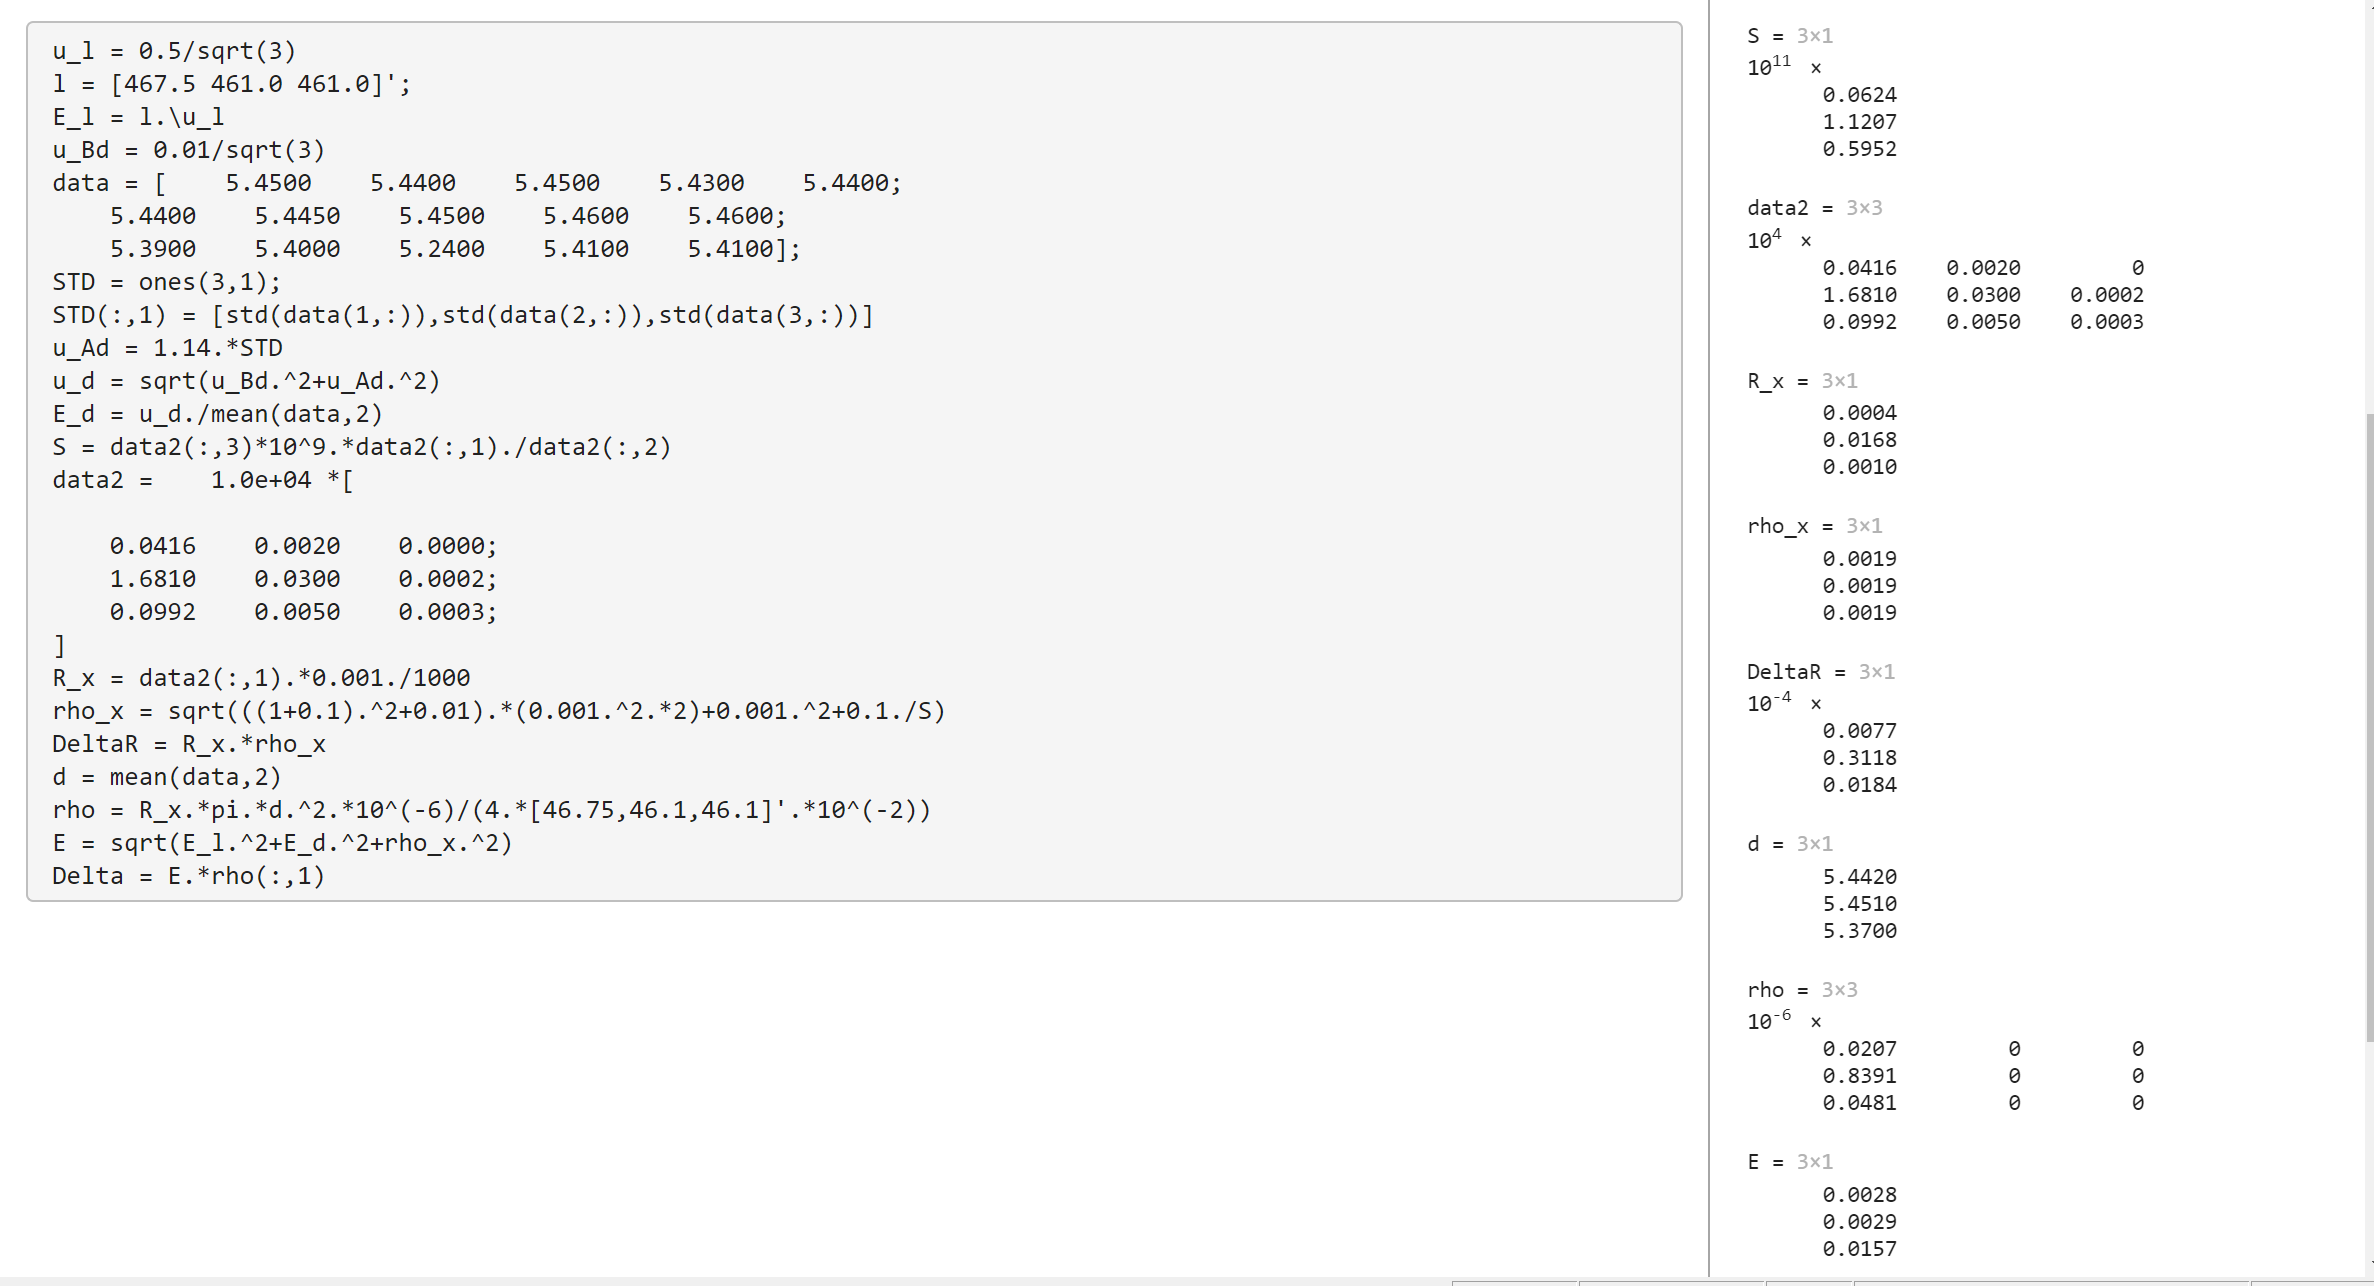
\includegraphics[width=1\textwidth]{计算过程}
	\end{figure}


\end{document}
